\documentclass{report}

\usepackage{xcolor}
\usepackage{indentfirst}
\usepackage{graphicx}
\usepackage{hyperref}
\usepackage{float}
\usepackage{wrapfig}

\begin{document}
  \section*{Question 1}
    \subsection*{a}
      Assuming the rules are to stuff a $0$ after five consecutive $1$'s, 
      and to encapsulate the entire message with $01111110$,
      the bits streamed are

      ${\color{blue}01111110}100011111{\color{blue}0}10100011111{\color{blue}0}011{\color{blue}01111110}$.
    \subsection*{b}
      The original bits are $11111110001111111$.
  
  \section*{Question 2}
    \subsection*{a}
      The encoded message is ${\color{blue}0}{\color{blue}1}1{\color{blue}0}001{\color{blue}1}1011$
      as derive from follows
      \begin{center}
        \begin{tabular}{|c|c|c|c|c|c|c|c|c|c|c|c|c|c|}
          \hline
          &1 (p1)&2 (p2)&3&4 (p3)&5&6&7&8 (p4)&9&10&11&12\\
          \hline
          &0&1&1&0&0&0&1&1&1&0&1&1 \\
          \hline
          p1&x& &x& &x& &x& &x& &x& \\
          \hline
          p2& &x&x& & &x&x& & &x&x& \\
          \hline
          p3& & & &x&x&x&x& & & & &x \\
          \hline
          p4& & & & & & & &x&x&x&x&x \\ 
          \hline
        \end{tabular}
      \end{center}
    \subsection*{b}
      \subsubsection*{i}
        Parity bits $p1$ and $p4$ are wrong, which suggests a flipped bit at
        $(1001)_2 = (9)_{10}^{th}$ bit 
      \subsubsection*{ii}
        Parity bits $p1$, $p2$ and $p4$ are wrong, which suggests a flipped bit at
        $(1011)_2 = (11)_{10}^{th}$ bit 
  
  \section*{3}
    \subsection*{a}
      As $C(x) = 10101$, the long division of $10110$ against $10101$ yields
      a remainder of $1111$. Thus, the encoded message is $10110{\color{blue}1111}$.
    \subsection*{b}
      \subsubsection*{i}
        The remainder is non-zero, the message is corrupted.
      \subsubsection*{ii}
        The remainer is zero, the message is intact.

  \section*{4}
    \begin{center}
      \begin{tabular}{|c|c|c|}
        \hline
        Destination&Cost&Next Hop \\
        \hline
        A&9&D \\
        \hline
        B&5&B \\
        \hline
        C&0&- \\
        \hline
        D&5&D \\
        \hline
        E&4&E \\
        \hline
        F&9&E \\
        \hline
      \end{tabular}
    \end{center}

  \section*{5}
    $time = (2^{64} \times 8)/(100 \times 1024^{4}) = 1342177\ s = 15\ days$

  \section*{6}
    According to figure \ref{fig:question6}, the domain was registered on 02-Jun-1986
    and will expire on 31-Jul-2024. It contains $3$ DNS servers: 
    \url{DNS-NC1-01.OIT.DUKE.EDU}, \url{DNS-AUTH-01.OIT.DUKE.EDU}, \url{DNS-AUTH-02.OIT.DUKE.EDU}
    \begin{figure}[ht]
      \centering
      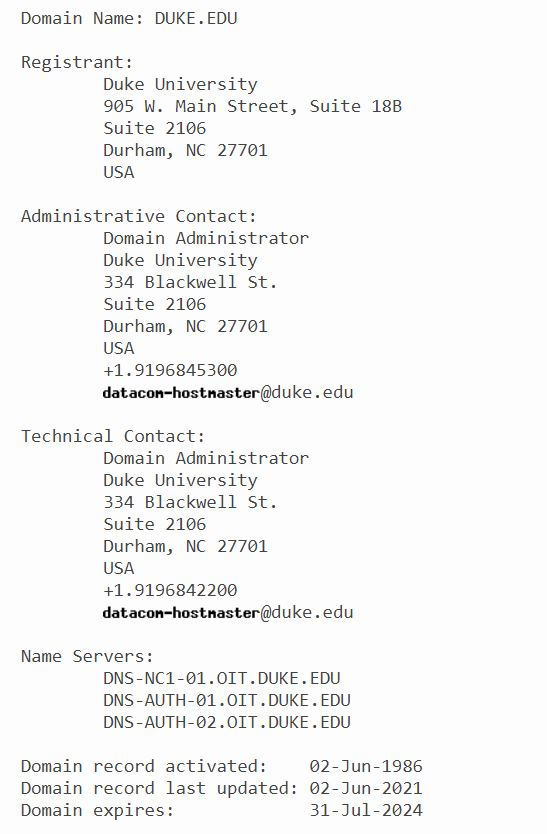
\includegraphics[width=0.9\textwidth]{images/question6.JPG}
      \caption{whois lookup result for \url{duke.edu}, from \url{https://www.whois.com/}}
      \label{fig:question6}
    \end{figure}
    

  \section*{7}
    The acquired response is as follows in figure \ref{fig:question7}.
    \begin{figure}[H]
      \centering
      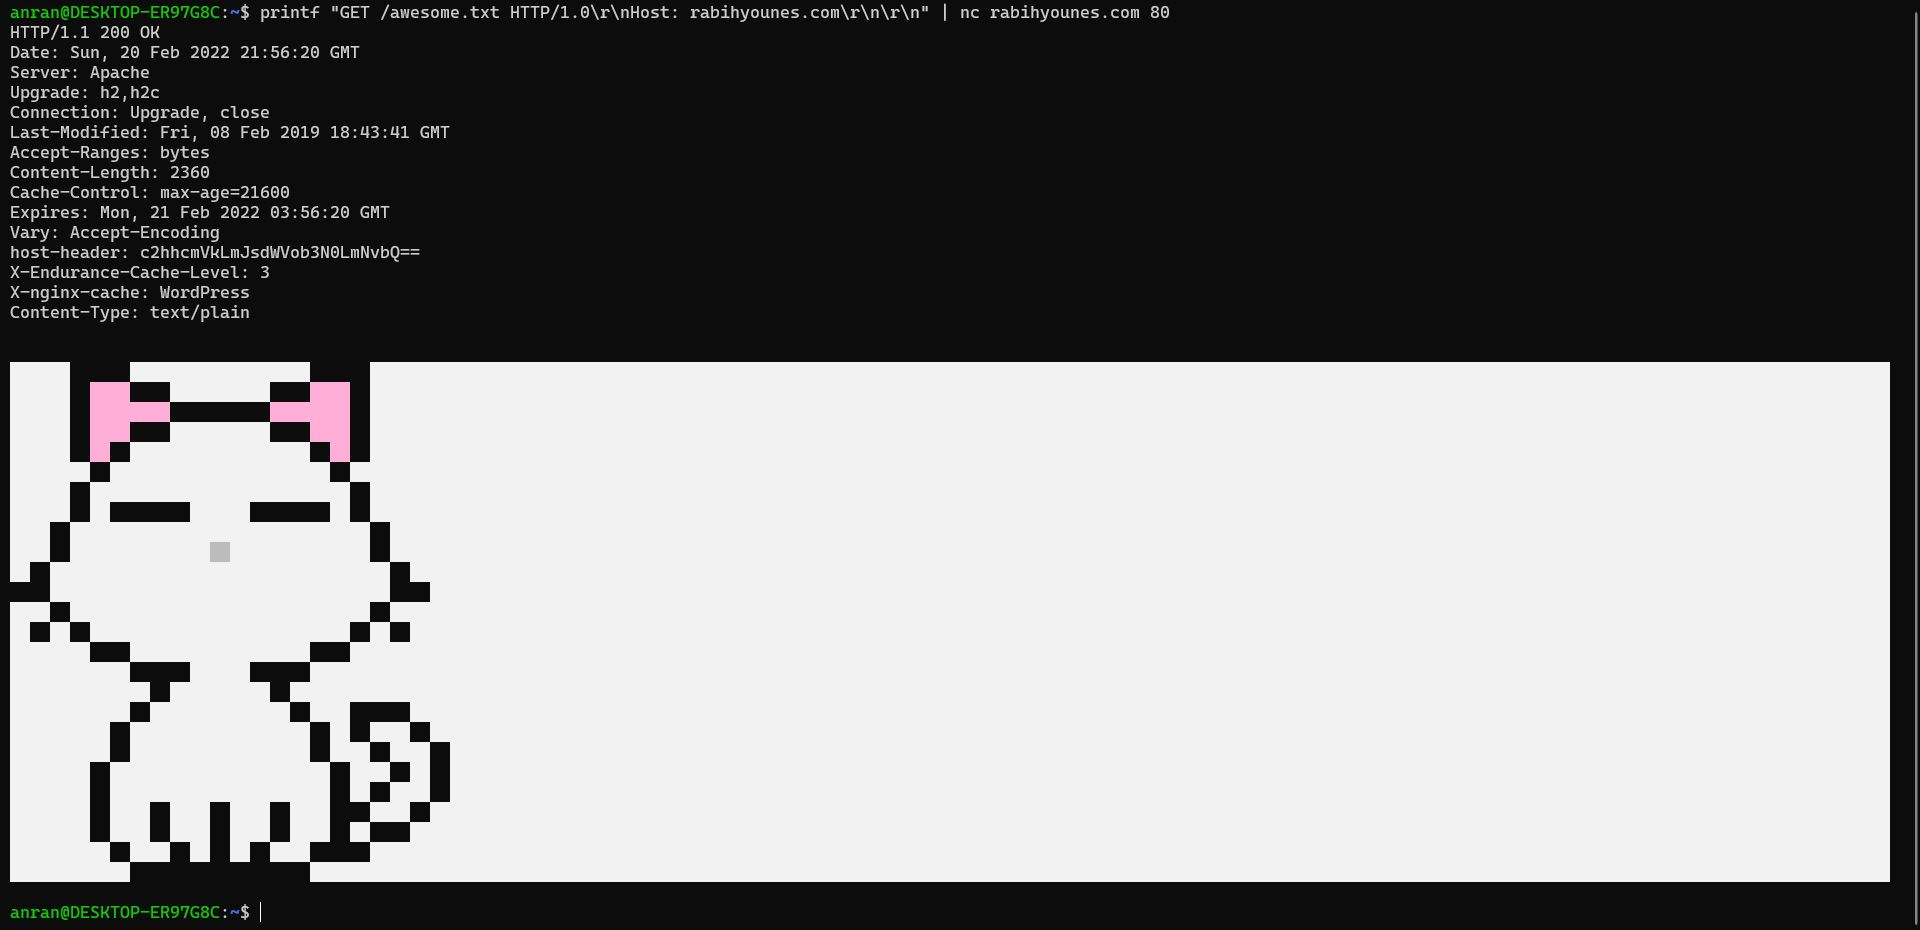
\includegraphics[width=0.9\textwidth]{images/question7.JPG}
      \caption{acquired message from \url{http://rabihyounes.com/awesome.txt}}
      \label{fig:question7}
    \end{figure}
\end{document}